\section{Propuesta de Solución}

En respuesta al contexto planteado anteriormente, se propone desarrollar un sistema automatizado para el monitoreo periódico de los parámetros de calidad del agua en cuerpos de agua que se mueven en una sola dirección, como ríos, riachuelos y arroyos. Este sistema integrará una red inalámbrica de sensores distribuidos, junto con un módulo de visión artificial para la detección de posibles residuos sólidos flotantes, como plásticos (PET), envases Tetra Pak, latas o desechos de unicel de un solo uso. La visión artificial procesará imágenes capturadas en intervalos de tiempo predefinidos, lo que permitirá estimar la cantidad de contaminantes flotantes presentes en la superficie del agua. Los sensores medirán parámetros clave de calidad del agua, incluyendo pH, oxigenación, temperatura, turbidez y conductividad, proporcionando información sobre su composición físico-química de forma periódica.

En la figura \ref{Dig:diagrama general} se presenta un diagrama a que muestra el funcionamiento general del sistema, destacando los diferentes módulos que lo componen: nodos sensores, nodo concentrador, almacenamiento en un servidor, así como la visualización a través de la página web.

\begin{figure}[H]
    \centering
    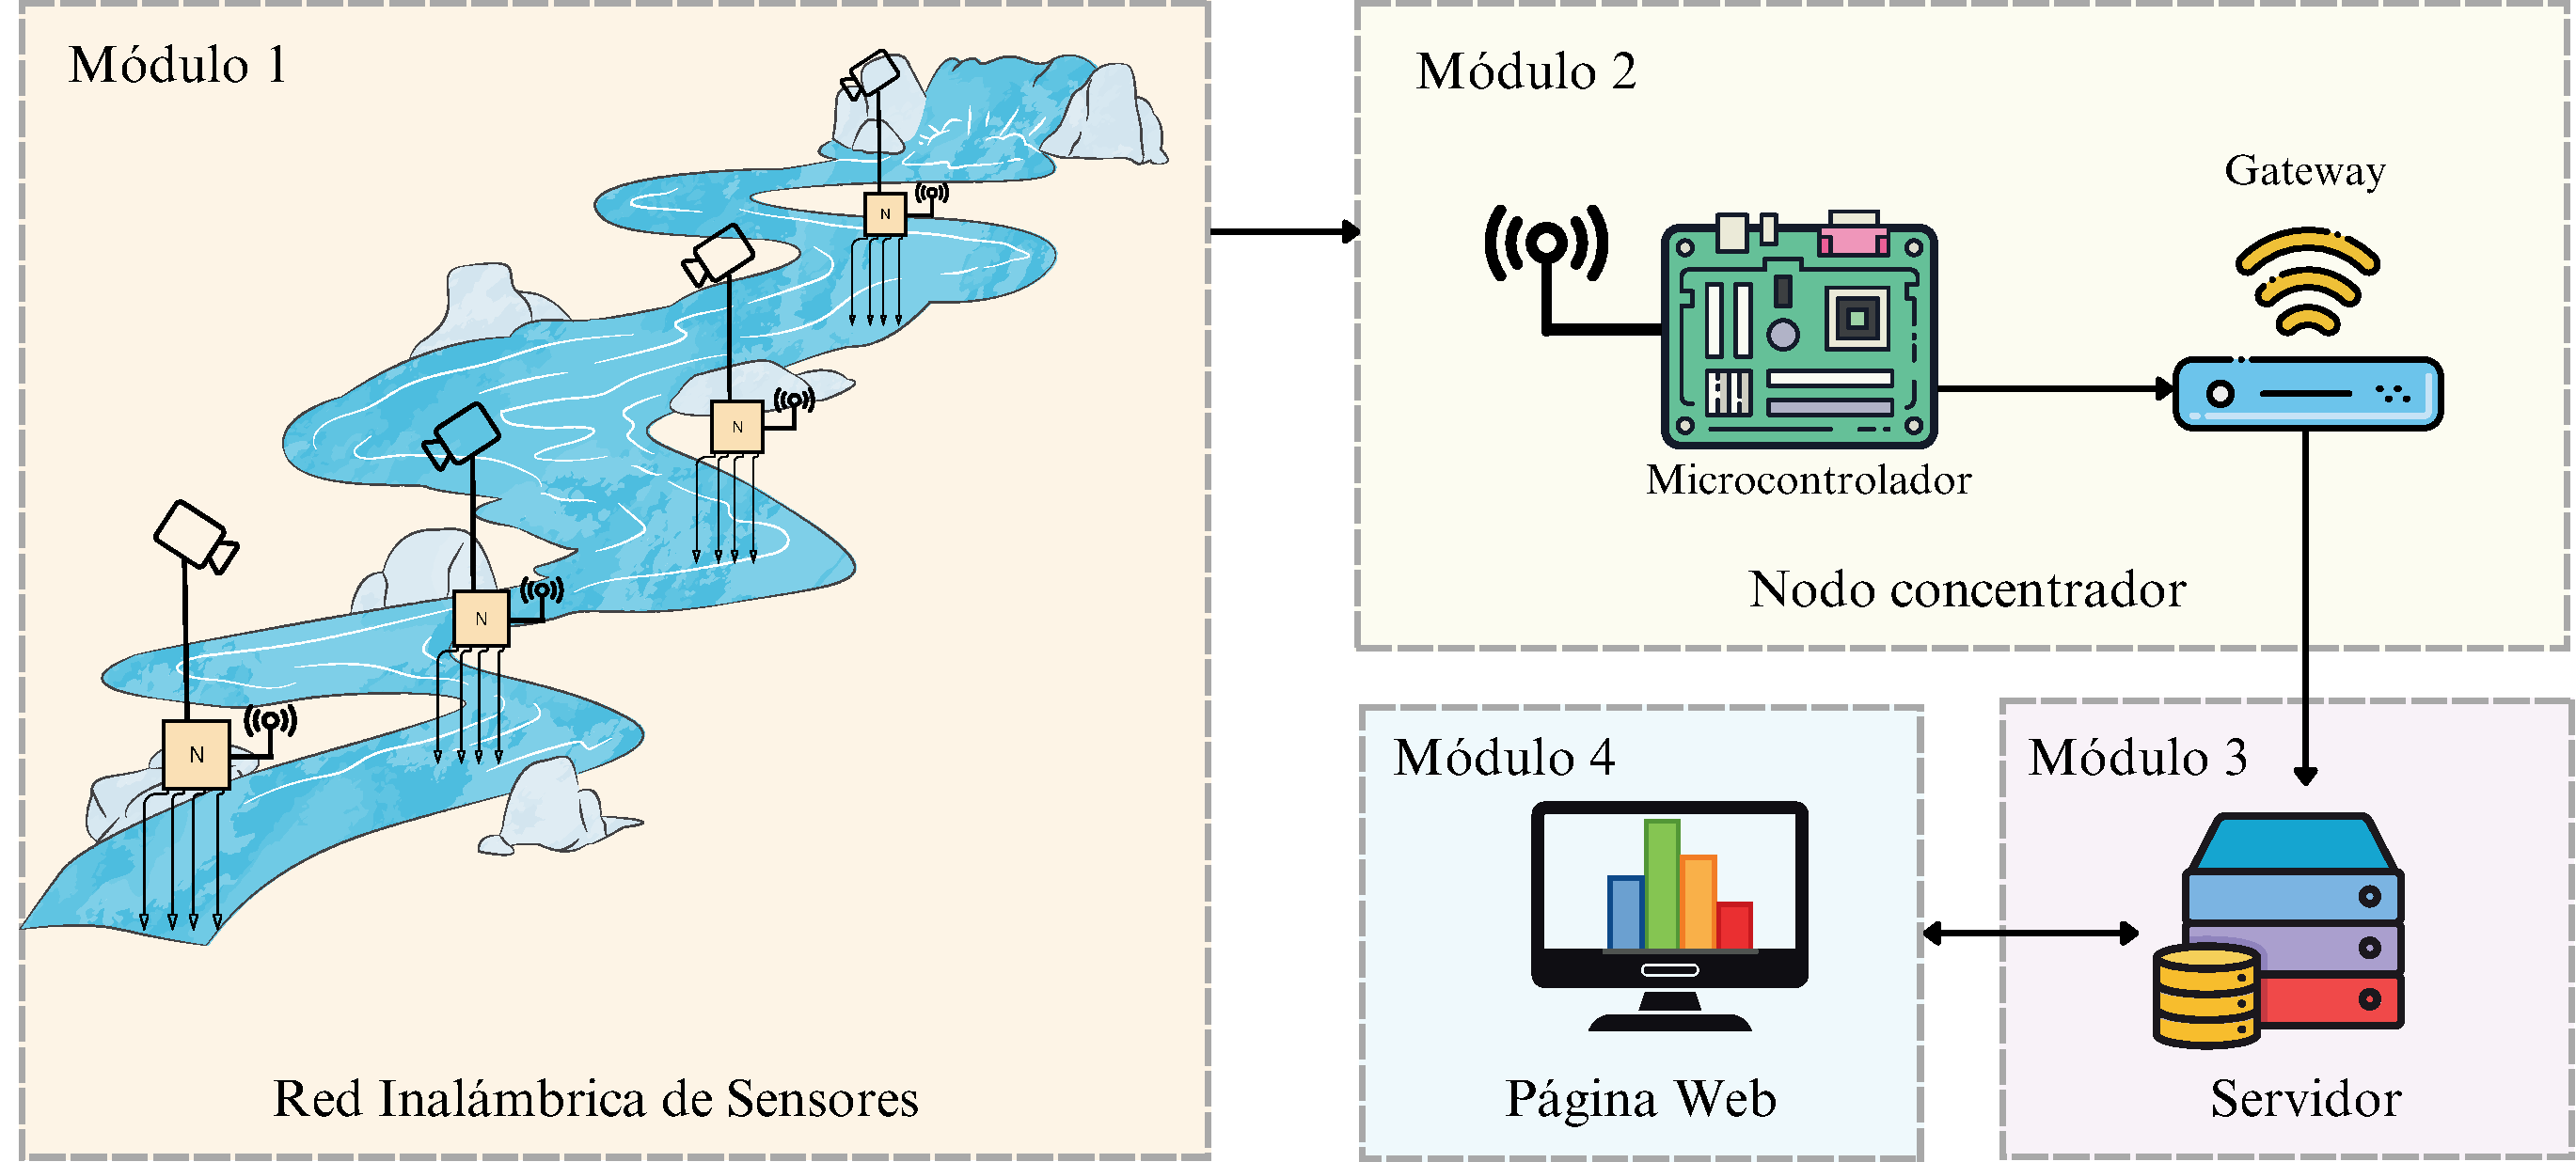
\includegraphics[width=0.9\textwidth]{Documento/Imagenes/Propuesta Sol/Dig_gen.pdf}
    \caption{Diagrama general del sistema.}
    \label{Dig:diagrama general}
\end{figure}


El diseño del sistema  considera las recomendaciones establecidas con las normas \textit{NTC-ISO 5667-1} y \textit{NTC-ISO 5667-10}, que recomiendan el uso de instrumentos automáticos en línea o muestreos regulares para obtener datos representativos. En este marco, la red de sensores con transmisión remota asegura mayor frecuencia y calidad en la información recolectada.  

La frecuencia inicial de monitoreo propúesta es mensual, con posibilidad de reducir intervalos según resultados y recursos, en coherencia con la \textit{NOM-001-SEMARNAT-2021} cuyas exigencias para descargas (municipales y no municipales) varían entre frecuencias mensuales, trimestrales o semestrales según el tipo de carga contaminante \cite{nom001}. Los datos se enviarán a un servidor central para su análisis y publicación en una plataforma web accesible a autoridades y comunidad, esta página permitirá la visualización de la información recopilada sobre la calidad del agua y las condiciones del cuerpo hídrico monitoreado.  

El sistema requiere conectividad de red estable, capacidad de almacenamiento y sensores con protección robusta (IP68/NEMA 6P) frente a condiciones adversas. Además, responde al mandato de la \textit{Ley de Aguas Nacionales} (Art. 86), que designa a la Autoridad del Agua promover, ejecutar y operar sistemas de monitoreo para preservar y mejorar la calidad del agua en cuencas y acuíferos \cite{LAN2024}, al habilitar un monitoreo hídrico constante, confiable y distribuido espacialmente.


\subsection{Módulo 1. Red Inalámbrica de Sensores}
Este módulo consiste en una red inalámbrica de cuatro nodos sensores distribuidos a lo largo del cuerpo de agua. Su función principal es realizar mediciones continuas de parámetros de calidad del agua y detectar residuos sólidos flotantes. La distancia entre nodos dependerá de la tecnología de transmisión empleada.

\subsubsection*{Red}
En aplicaciones ribereñas con cobertura longitudinal, la topología lineal/semi-lineal es esencial, requiriendo comunicación confiable entre nodos adyacentes para transferencias eficientes a lo largo del cauce.

\subsubsection*{Nodos Sensores}
\begin{itemize}  
  \item \textbf{Sensores:} Para medir pH, temperatura, turbidez, oxígeno disuelto y conductividad.
  \item \textbf{Microcontrolador:}Gestiona la adquisición de datos, comunicación y un sistema de visión artificial para detectar residuos sólidos flotantes.
  \item \textbf{Comunicación inalámbrica:} El dispositivo permite enviar y recibir datos para comunicarse con otros dispositivos dentro de su rango.
  \item \textbf{Visión artificial:} Módulo óptico para detección de residuos, con efectividad condicionada a la luz natural. Se evaluarán algoritmos eficientes entrenados para entornos fluviales.
  \item \textbf{Alimentación:} Sistema autónomo mediante baterías y/o paneles solares para alimentar todos los componentes.
\end{itemize}

\subsection{Módulo 2. Nodo Concentrador}
El nodo concentrador actúa como puente entre la red de sensores y el servidor central, cumpliendo una función dual: opera como un nodo sensor estándar y como punto de agregación y comunicación con el servidor.

\begin{itemize}
  \item \textbf{Hardware}
  \item \textbf{Control}
  \item \textbf{Flujo}
\end{itemize}

\subsection{Módulo 3. Servidor}
Es el centro de procesamiento y gestión, compuesto por:
\begin{itemize}
\item \textbf{Base de Datos:} Almacena las series temporales de los parámetros medidos.
\item \textbf{Backend:} Realiza el procesamiento analítico (ej., detección de anomalías).
\item \textbf{Frontend Web:} Sirve la interfaz de usuario para la visualización.
\end{itemize}

\subsection{Módulo 4. Interfaz Web de Monitoreo}
Plataforma web pública y de acceso libre que muestra:
\begin{itemize}
\item \textbf{Calidad del Agua:} Gráficos de series temporales de los parámetros con indicadores de estado.
\item \textbf{Basura Flotante:} Frecuencia de detecciones e histórico de eventos.
\end{itemize}


\begin{comment}
El diseño del sistema considera las recomendaciones establecidas en las normas \textit{NTC-ISO 5667-1} y \textit{NTC-ISO 5667-10}, las cuales reconocen que la variabilidad aleatoria y sistemática en las concentraciones de contaminantes dificulta obtener resultados representativos mediante muestreo manual puntual. Por ello, se recomienda el uso de instrumentos automáticos en línea (on-line) capaces de suministrar análisis continuos \cite{iso5667-10}, o bien realizar muestreos compuestos a intervalos regulares cuando no se dispone de dicha tecnología \cite{iso5667}. En este sentido, la implementación de una red de sensores con capacidad de transmisión remota representa una alternativa alineada a estas directrices normativas y mejora significativamente la frecuencia, oportunidad y calidad de los datos obtenidos.

La frecuencia de monitoreo inicial propuesta es mensual, sustentada en criterios técnicos, operativos y normativos. No obstante, la arquitectura automatizada del sistema permite operar en intervalos menores si se requieren. Esta periodicidad se ajustará conforme al análisis de resultados y disponibilidad de recursos durante la implementación, y resulta coherente con la \textit{NOM-001-SEMARNAT-2021}, cuyas exigencias para descargas (municipales y no municipales) varían entre frecuencias mensuales, trimestrales o semestrales según el tipo de carga contaminante \cite{nom001}.


El sistema transmitirá periódicamente los datos a una central de procesamiento, donde serán analizados y posteriormente publicados en una plataforma web accesible. Esta página permitirá la visualización de la información recopilada sobre la calidad del agua y las condiciones del cuerpo hídrico monitoreado a los interesados como autoridades, personas que residen cerca de los cuerpos de agua y público en general.
La información recopilada se procesará y almacenará en un servidor seguro, para luego publicarse en una plataforma web de interfaz intuitiva y accesibilidad universal.


La implementación exitosa exige dos prerrequisitos funcionales: conectividad de red estable para la transmisión continua de datos e infraestructura de almacenamiento con capacidad de procesamiento. Además, los módulos sensores deben integrar protección robusta (IP68/NEMA 6P) contra agentes hidrodinámicos (corrientes rápidas), exposición química (pH extremo, contaminantes), variables termohigrométricas (humedad, fluctuaciones térmicas) y turbidez elevada, garantizando operatividad confiable y durabilidad en ambientes acuáticos adversos.

Además de abordar necesidades técnicas y ambientales, este sistema cumple con lo establecido en la \textit{Ley de Aguas Nacionales} (Artículo 86), que designa a la Autoridad del Agua promover, ejecutar y operar sistemas de monitoreo para preservar y mejorar la calidad del agua en cuencas y acuíferos \cite{LAN2024}. La propuesta aquí desarrollada contribuye directamente a este mandato legal, ofreciendo una herramienta automatizada que habilita una supervisión hídrica constante, precisa y distribuida espacialmente.

\subsection{Módulo 1. Red Inalámbrica de Sensores}

Este módulo está conformado por una red inalámbrica de sensores, integrada por cuatro nodos sensores distribuidos a lo largo del cuerpo de agua, cuya distancia entre ellos dependerá de la tecnología empleada para la transmisión de datos. Su función principal es realizar mediciones continuas de parámetros de calidad del agua y la detección de residuos sólidos flotantes.


\subsubsection*{\textbf{Red}}

En aplicaciones ribereñas que demandan cobertura longitudinal, la topología lineal/semi-lineal resulta estratégica, influyendo tanto en el diseño del hardware como en la transmisión de datos. En tales escenarios, garantizar una comunicación confiable entre nodos adyacentes es requisito indispensable para transferencias de datos eficientes a lo largo del cauce.

\subsubsection*{\textbf{Nodos Sensores}}

Cada nodo sensor integrará sensores especializados para medir parámetros esenciales de calidad del agua como pH, temperatura, turbidez, oxígeno disuelto y conductividad. El nodo sensor incluye los componentes fundamentales: un microcontrolador, un transceptor inalámbrico, una fuente de alimentación y una cámara, todos interconectados y con capacidad de transmisión de datos remota. 

\begin{itemize}
    \item \textbf{Microcontrolador:} Opera como unidad central gestionando: la adquisición multisensorial, captura de imágenes para visión artificial, y comunicación inter-nodal bidireccional; coordinando el preprocesamiento local y enrutamiento de datos hacia nodos vecinos.
    \item \textbf{Sensores:} Se tendrán sensores que producen una respuesta medible de los parámetros a sensar como el pH, oxigenación, turbidez, temperatura y conductividad en el área de monitoreo.
    
Algunas características a considerar para los sensores: 
    \begin{itemize}
        \item Precisión y sensibilidad: Deben proporcionar mediciones exactas y detectar pequeñas variaciones en los parámetros.
        \item Tamaño compacto: Permite su instalación en un entorno natural variante y manipulación para ajuste.
        \item Materiales resistentes: garantiza la durabilidad del sensor en condiciones adversas.
        \item Bajo consumo energético: Fundamental para su uso en sistemas remotos o alimentados por baterías.
        \item Compatibilidad con sistemas inalámbricos: Para transmitir datos a un servidor o estación base de forma eficiente.
    \end{itemize}    


\item \textbf{Comunicación Inalámbrica:} El dispositivo permite enviar y recibir datos para comunicarse con otros dispositivos dentro de su rango.
    
\item \textbf{Sistema de Visión Artificial:} Emplea un módulo de captura óptica para monitorear la superficie acuática, especializado en la detección de residuos sólidos flotantes. La efectividad del proceso está condicionada a la disponibilidad de luz diurna, factor crítico para garantizar la confiabilidad métrica. Dada esta dependencia, la selección del algoritmo de clasificación resulta determinante para optimizar la precisión del sistema. Se evaluarán arquitecturas eficientes en entornos embebidos (e.g., YOLO, MobileNet) y modelos basados en redes convolucionales, entrenados con datasets específicos de residuos en contextos fluviales.


\item \textbf{Alimentación:} La fuente de alimentación debe ser capaz de alimentar a los sensores, las cámaras, el procesamiento y la comunicación, ya que no se dispone de red eléctrica, hay opciones como baterías y/o mediante placas solares.

\end{itemize}
\subsection{Módulo 2. Nodo Concentrador}
El nodo concentrador opera como punto terminal de la red inalámbrica y nodo sensor avanzado, integrando capacidades adicionales de gestión y comunicación. Cumple una función dual: como elemento sensorial equivalente a los nodos del Módulo 1, y como puente de comunicaciones hacia el servidor central. Su diseño garantiza interoperabilidad completa con la arquitectura de red establecida.

\begin{itemize}
    \item \textbf{Funcionalidad Dual:} 
    Opera simultáneamente como: 
    (i) nodo sensor estándar (adquiriendo parámetros de calidad del agua mediante sensores especializados y detectando residuos con visión artificial), 
    (ii) punto de agregación de datos de la red, y 
    (iii) interfaz de comunicación con el servidor central.
    
    \item \textbf{Arquitectura Hardware:} 
    Mantiene los componentes básicos de los nodos sensores (microcontrolador, transceptor inalámbrico, fuente de alimentación, sensores y módulo de visión artificial), pero incorpora:
    \begin{itemize}
        \item Módulo de comunicación backhaul para conectividad con el servidor.
        \item Memoria ampliada para almacenamiento temporal de datos agregados.
    \end{itemize}
    
    \item \textbf{Microcontrolador:} 
    Requiere especificaciones mejoradas para gestionar:
    \begin{itemize}
        \item Procesamiento concurrente de datos locales y remotos.
        \item Protocolos de comunicación múltiples (intra-red + backhaul).
        \item Mecanismos de priorización de tráfico.
    \end{itemize}
    
    \item \textbf{Flujo de Datos:} 
    Implementa un pipeline de procesamiento donde:
    \begin{enumerate}
        \item Recibe datos de nodos precedentes mediante el protocolo de red.
        \item Agrega información local (sensórica y/o visual).
        \item Organiza paquetes mediante esquemas de codificación eficiente.
        \item Transmite datos consolidados al servidor mediante el canal backhaul.
    \end{enumerate}
    
    \item \textbf{Comunicaciones:} 
    Emplea dos interfaces diferenciadas:
    \begin{itemize}
        \item \textbf{Intra-red:} Transceptor para comunicación con nodos sensores en topología lineal.
        \item \textbf{Backhaul:} Módulo para transmisión al servidor, con mecanismos de retransmisión y QoS adaptativos
    \end{itemize}
\end{itemize}


\subsection{Módulo 3. Servidor}
El servidor central constituye la capa de gestión y presentación del sistema, integrando tres componentes fundamentales: (i) servidor de base de datos para almacenamiento estructurado, (ii) backend de procesamiento analítico, y (iii) frontend web para visualización interactiva. Opera como repositorio centralizado y punto de acceso para monitoreo ambiental.

\begin{itemize}
    \item \textbf{Arquitectura Integrada:}
    \begin{itemize}
        \item \textbf{Servidor de Base de Datos:} Aloja el sistema de gestión de bases de datos (SGBD) relacional para almacenamiento estructurado de:
        \begin{itemize}
            \item Series temporales de parámetros fisicoquímicos
            \item Metadatos de detección de residuos
        \end{itemize}
       \item \textbf{Servidor de Aplicaciones y Web:} 
            Combina la lógica de procesamiento y la capa de presentación en una arquitectura unificada:
            \begin{itemize}
                \item \textit{Backend (Lógica de Negocio):}
                \begin{itemize}
                    \item Ejecuta procesamiento analítico avanzado (correlación de datos, detección de anomalías)
                    \item Gestiona APIs RESTful para comunicación interna/externa
                    \item Administra servicios de autenticación y seguridad
                \end{itemize}
                
                \item \textit{Frontend (Interfaz de Usuario):}
                \begin{itemize}
                    \item Hospeda aplicación web basada en tecnologías modernas (HTML5/CSS3/JavaScript)
                    \item Implementa dashboards interactivos para visualización de datos
                    \item Garantiza experiencia responsive para múltiples dispositivos
                \end{itemize}
        \end{itemize}
    \end{itemize}

    \item \textbf{Flujo de Información:}
    \begin{enumerate}
        \item Recepción de datos consolidados desde el nodo concentrador
        \item Validación y almacenamiento en el SGBD
        \item Procesamiento analítico en el servidor de aplicaciones
        \item Presentación mediante el servidor web a usuarios finales
    \end{enumerate}
\end{itemize}


\subsection{Módulo 4. Interfaz Web de Monitoreo}
Plataforma web de acceso público diseñada para visualizar parámetros de calidad del agua y eventos de detección de basura flotante. Proporciona un dashboard intuitivo, con acceso libre sin requerimiento de autenticación.

\begin{itemize}
    \item \textbf{Arquitectura y Acceso:}
    \begin{itemize}
        \item Diseño responsive basado en frameworks
        \item Acceso universal sin registro
        \item Interfaz simplificada con navegación intuitiva
    \end{itemize}
    
    \item \textbf{Visualización de Parámetros de Calidad del Agua:}
    \begin{itemize}
        \item Gráficos dinámicos de series temporales (pH, temperatura, turbidez, oxígeno disuelto, conductividad)
        \item Paneles comparativos entre diferentes periodos
        \item Indicadores de estado actual con semaforización (normal/advertencia/crítico)
    \end{itemize}
    
    \item \textbf{Monitoreo de Basura Flotante:}
    \begin{itemize}
        \item Indicadores binarios de presencia/ausencia de residuos
        \item Gráficos de frecuencia de detecciones (eventos/hora, eventos/día)
        \item Histórico de eventos con timestamps
        \item Indicadores de confianza promedio en las detecciones
    \end{itemize}
\end{itemize}
\end{comment}

\section{Alcances}
Los aspectos por considerar para el funcionamiento del sistema son los siguientes:

\begin{itemize}

    \item La red inalámbrica contará con al menos 4 nodos sensores, los cuales serán ubicados estratégicamente según la distancia de cobertura entre sensores. Estos nodos permitirán monitorear parámetros como pH, temperatura, turbidez, oxígeno disuelto y conductividad en diferentes puntos del cuerpo de agua.

    \item La comunicación entre los nodos sensores se establecerá con una distancia de al menos 50 metros, mientras que la distancia máxima dependerá de las características topográficas del área de implementación. Se propone el uso de una topología lineal o semi-lineal, dependiendo de la zona del cuerpo de agua elegida para monitorear y su entorno, adaptada al entorno, con la posibilidad de ampliar la cobertura de la red mediante configuraciones más complejas.
    
    \item El sistema de visión artificial detectará exclusivamente residuos sólidos en la superficie del agua; no se identificarán tipos de contaminantes sumergidos o invisibles al rango de la cámara.
    
    \item El sistema no reemplazará la toma de decisiones humanas; su objetivo será únicamente proporcionar información accesible a través de una página web, facilitando al público la comprensión del estado de los cuerpos de agua monitoreados.
    \item El sistema se limitará únicamente al monitoreo de parámetros de calidad del agua y a la detección de residuos sólidos flotantes. No realizará ningún tipo de separación, recolección o tratamiento de los residuos identificados.

\end{itemize}
